\documentclass[12pt]{article}

\usepackage{graphicx}
\usepackage{xcolor}

\definecolor{ncertblue}{RGB}{0,153,204}

\begin{document}

\raggedright
\setlength{\parindent}{0pt}
\setlength{\parskip}{0.5\baselineskip}

\begin{center}

\includegraphics[width=4cm]{iiitb_comet_logo.jpg}

\textbf{Srinidhi A}

\textbf{ID: COMETFWC053}
\end{center}

\begin{center}
\textcolor{ncertblue}{\textbf{EXERCISE 2.1}}
\end{center}

\begin{enumerate}
\item The graphs of $y = p(x)$ are given in Fig. 2.10 below, for some polynomials $p(x)$. Find the number of zeroes of $p(x)$, in each case.
\end{enumerate}

\begin{center}
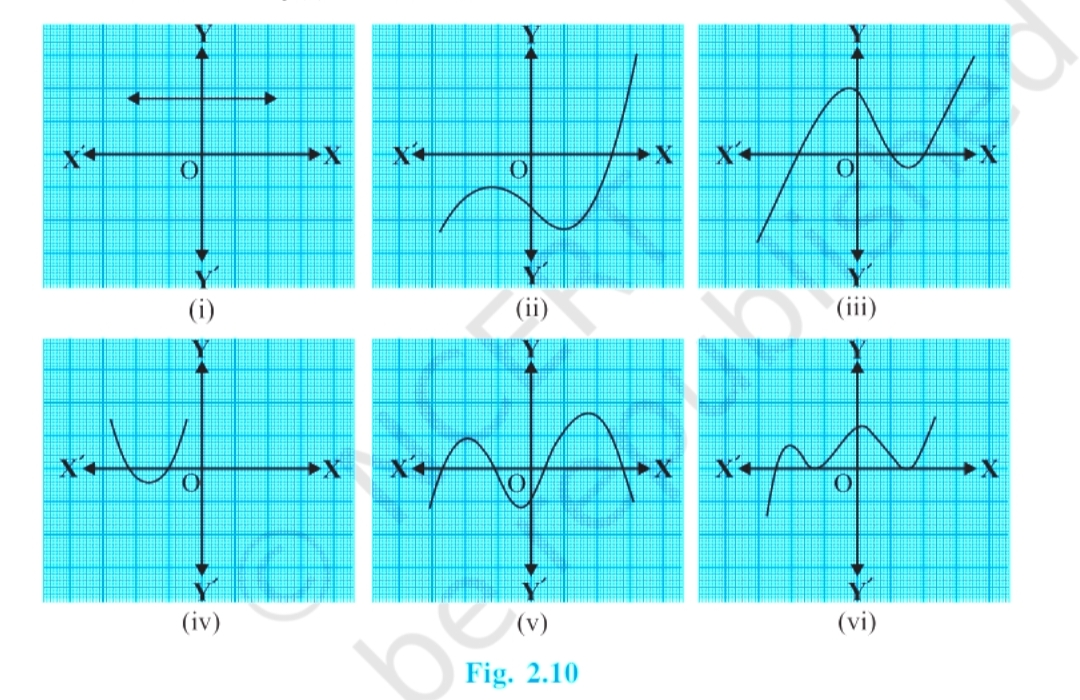
\includegraphics[width=0.9\textwidth]{fig_2_10.jpg}

Fig. 2.10
\end{center}

\newpage

\textcolor{ncertblue}{\textbf{Example 4:}}
Find a quadratic polynomial, the sum and product of whose zeroes are $-3$ and $2$, respectively.

\textcolor{ncertblue}{\textbf{Solution:}}
Let the quadratic polynomial be $ax^2 + bx + c$ and its zeroes be $\alpha$ and $\beta$.

We have $\alpha + \beta = -3 = -\frac{b}{a}$ and $\alpha\beta = 2 = \frac{c}{a}$.

If $a = 1$, then $b = 3$ and $c = 2$.

So, one quadratic polynomial which fits the given conditions is  
$x^2 + 3x + 2$.

You can check that any other quadratic polynomial which fits these conditions will be of the form  
$k(x^2 + 3x + 2)$, where $k$ is a real number.

Let us now look at cubic polynomials.  
Do you think a similar relation holds between the zeroes of a cubic polynomial and its coefficients?

Let us consider $p(x) = 2x^3 - 5x^2 - 14x + 8$.

You can check that $p(x) = 0$ for $x = 4$, $-2$ and $\frac{1}{2}$.  
Since $p(x)$ can have at most three zeroes, these are the zeroes of the given polynomial.

Now, the sum of the zeroes is  
$4 + (-2) + \frac{1}{2} = \frac{5}{2} = -\frac{\text{coefficient of } x^2}{\text{coefficient of } x^3}$.

The product of the zeroes is  
$4 \times (-2) \times \frac{1}{2} = -4 = -\frac{\text{constant term}}{\text{coefficient of } x^3}$.

The sum of the products of the zeroes taken two at a time is  
$(4 \times -2) + (-2 \times \frac{1}{2}) + (\frac{1}{2} \times 4) = -7  
= \frac{\text{coefficient of } x}{\text{coefficient of } x^3}$.

In general, if $\alpha$, $\beta$ and $\gamma$ are the zeroes of the cubic polynomial  
$ax^3 + bx^2 + cx + d$, then

$\alpha + \beta + \gamma = -\frac{b}{a}$  

$\alpha\beta + \beta\gamma + \gamma\alpha = \frac{c}{a}$  

$\alpha\beta\gamma = -\frac{d}{a}$.

\newpage

\textcolor{ncertblue}{\textbf{Example 5*:}}
Verify that $3$, $-1$ and $-\frac{1}{3}$ are the zeroes of the cubic polynomial  
$p(x) = 3x^3 - 5x^2 - 11x - 3$, and then verify the relationship between the zeroes and the coefficients.

\textcolor{ncertblue}{\textbf{Solution:}}
Comparing the given polynomial with $ax^3 + bx^2 + cx + d$, we get

$a = 3$, $b = -5$, $c = -11$ and $d = -3$.

Further,

$p(3) = 3(3)^3 - 5(3)^2 - 11(3) - 3  
= 81 - 45 - 33 - 3  
= 0$

$p(-1) = 3(-1)^3 - 5(-1)^2 - 11(-1) - 3  
= -3 - 5 + 11 - 3  
= 0$

$p\left(-\frac{1}{3}\right)
= 3\left(-\frac{1}{3}\right)^3 - 5\left(-\frac{1}{3}\right)^2 - 11\left(-\frac{1}{3}\right) - 3  
= -\frac{1}{9} - \frac{5}{9} + \frac{11}{3} - 3  
= 0$

Therefore, $3$, $-1$ and $-\frac{1}{3}$ are the zeroes of the given polynomial.

So, we take $\alpha = 3$, $\beta = -1$ and $\gamma = -\frac{1}{3}$.

Now,

$\alpha + \beta + \gamma
= 3 + (-1) + \left(-\frac{1}{3}\right)
= \frac{5}{3}
= -\frac{b}{a}$

$\alpha\beta + \beta\gamma + \gamma\alpha
= (3)(-1) + (-1)\left(-\frac{1}{3}\right) + \left(-\frac{1}{3}\right)(3)
= -3 + \frac{1}{3} - 1
= -\frac{11}{3}
= \frac{c}{a}$

$\alpha\beta\gamma
= (3)(-1)\left(-\frac{1}{3}\right)
= 1
= -\frac{d}{a}$

Hence, the relationship between the zeroes and the coefficients of the given cubic polynomial is verified.

\newpage

\textcolor{ncertblue}{\textbf{Example 6:}}
Divide $2x^2 + 3x + 1$ by $x + 2$.

\textcolor{ncertblue}{\textbf{Solution:}}
We stop the division process when either the remainder is zero or its degree is less than the degree of the divisor.

Here, the quotient is $2x - 1$ and the remainder is $3$.

Also,  
$(2x - 1)(x + 2) + 3 = 2x^2 + 3x + 1$.

That is,  
$2x^2 + 3x + 1 = (x + 2)(2x - 1) + 3$.

Therefore,  
Dividend = Divisor * Quotient + Remainder.

Let us now extend this process to divide a polynomial by a quadratic polynomial.

\end{document}
